\input ../preamble

\begin{document}

{\Huge

  \centerline{\bf TTIC 31230, Fundamentals of Deep Learning}
  \bigskip
  \centerline{David McAllester, April 2017}


\vfill
\centerline{\bf AlphaZero}
\vfill
\vfill

\slide{AlphaGo Fan (October 2015)}

AlphaGo Defeats Fan Hui, European Go Champion.

\vfill
\centerline{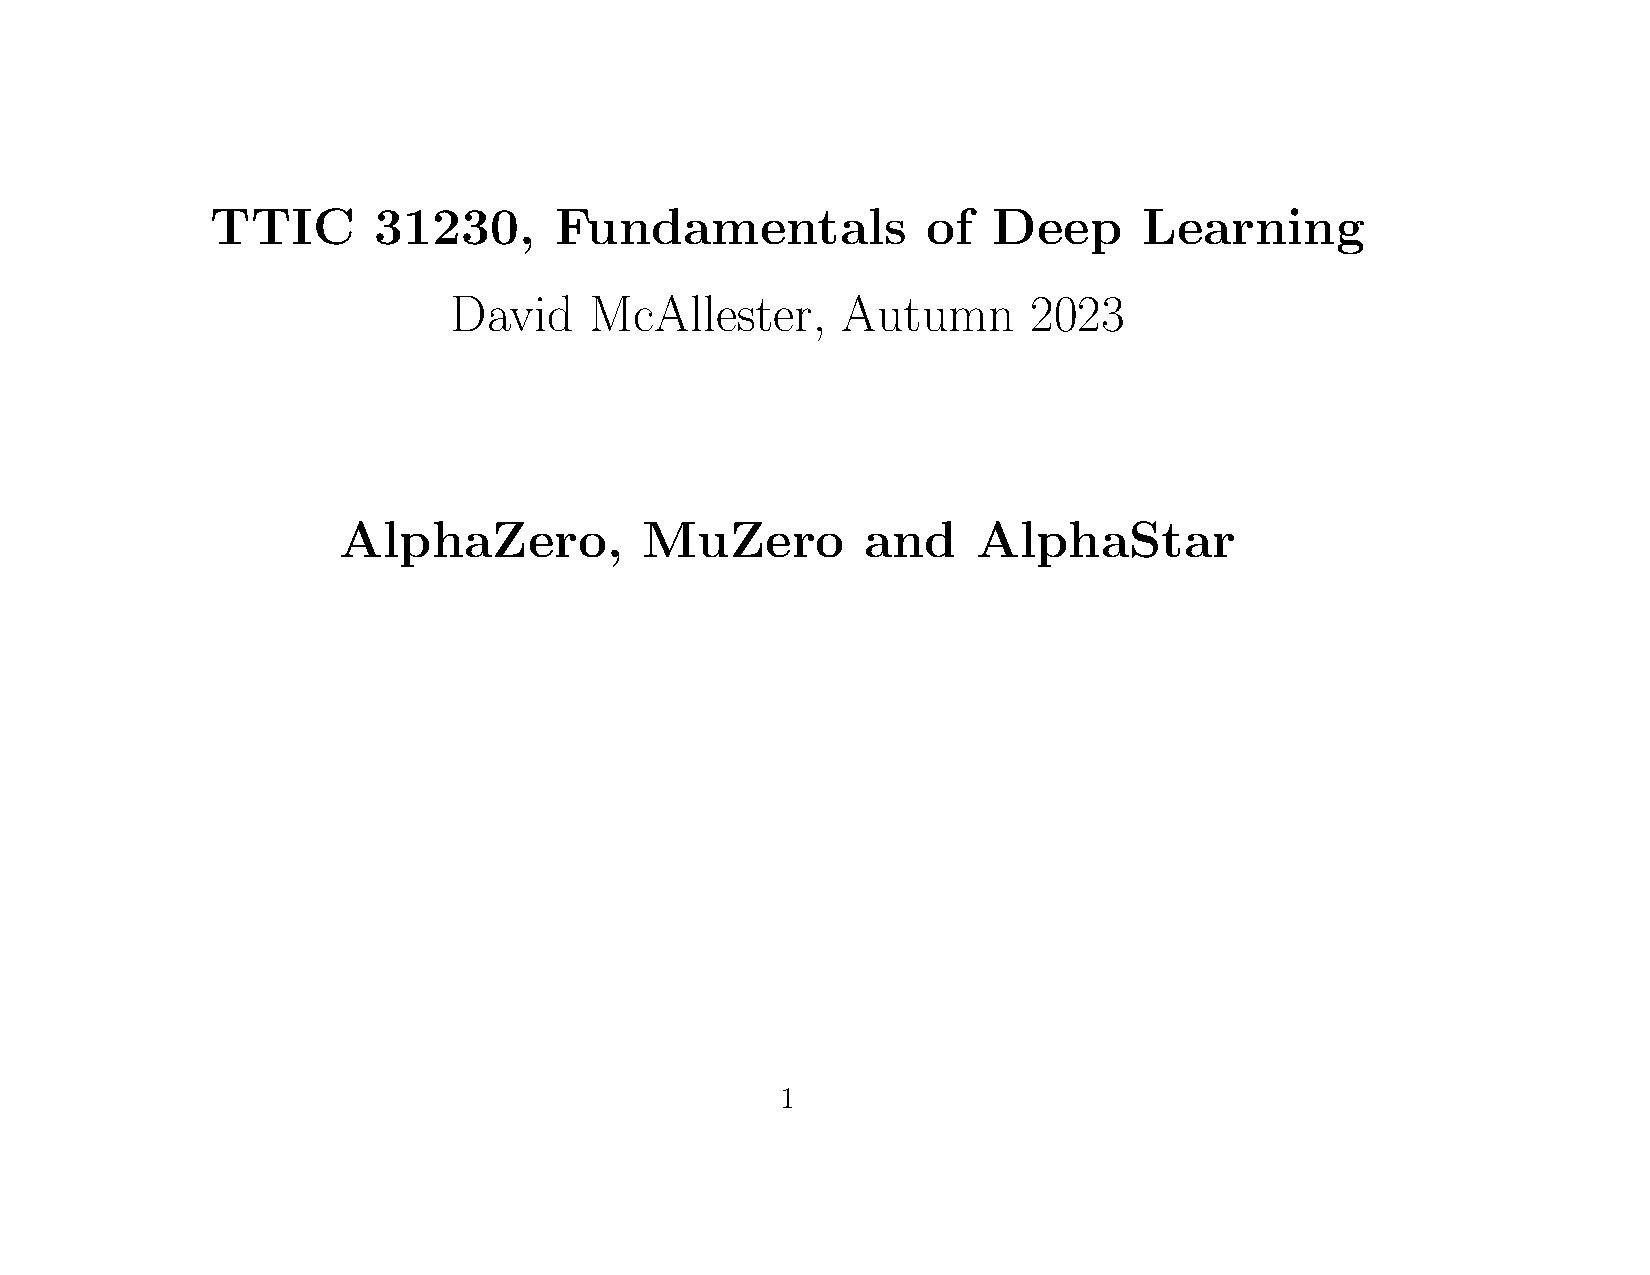
\includegraphics[width=4in]{../images/alphago}}

\slide{AlphaGo Lee (March 2016)}

\vfill
\centerline{\includegraphics[width=8in]{../images/alphalee}}

\slide{AlphaGo Zero vs. Alphago Lee (April 2017)}

{\bf AlphaGo Lee:}

\begin{itemize}
\item Trained on both human games and self play.
  
\item Trained for Months.

\item Run on many machines with 48 TPUs for Lee Sedol match.
\end{itemize}

{\bf AlphaGo Zero:}
\begin{itemize}
\item Trained on self play only.
  
\item Trained for 3 days.

\item Run on one machine with 4 TPUs.

\item Defeated AlphaGo Lee under match conditions 100 to 0.
\end{itemize}

\slide{AlphaZero Defeats Stockfish in Chess (December 2017)}

AlphaGo Zero was a fundamental algorithmic advance for general RL.

\vfill
The general RL algorithm of AlphaZero is essentially the same as that of AlphaGo Zero.

\slide{Some Algorithmic Concepts}

Rollout position evaluation (Bruegmann, 1993)

\vfill
Monte Carlo Tree Search (MCTS) (Bruegmann, 1993)

\vfill
Upper Confidence Bound (UCB) Bandit Algorithm (Lai and Robbins 1985)

\vfill
Upper Confidence Tree Search (UCT) (Kocsis and Szepesvari, 2006)

\slide{Rollouts and MCTS (1993)}

To estimate the value of a position (who is ahead and by how much)
run a cheap stochastic policy to generate a sequence of moves (a rollout) and see who wins.

\vfill
Take an average value of many rollouts.

\vfill
Do a selective tree search using rollout averages for position evaluation.

\slide{(One Armed) Bandit Problems}

Consider a set of choices (different slot machines).

Each choice gets a stochastic reward.

\vfill
We can select a choice and get a reward as often as we like.

\vfill
We would like to determine which choice is best and also to get reward as quickly as possible.

\slide{The UCB algorithm (1995 Version)}

For each choice (bandit) $a$ construct a confidence interval for its average reward.

\vfill
$$\mu = \hat{\mu} \pm 2\sigma/\sqrt{n}$$

\vfill
$$\mu(a) \leq \hat{\mu}(a) + U(N(a))$$

\vfill
Always select

$$\argmax_a \hat{\mu}(a) + U(N(a))$$

\slide{The UCT algorithm (2006)}

Build a search tree by running ``simulations''.

\vfill
Each simulation uses the UCB rule to select a child of each node until a leaf is reached.

\vfill
The leaf is then expanded and a value is computed for the leaf.

\vfill
This value is ``backed up'' through the tree adding a value and increment the count of each
ancestor node.

\slide{AlphaGo}

AlphaGo trained:

\begin{itemize}
\item a fast rollout policy.

\item an imitation policy network.

\item a self-play policy network.

\item a value network trained to predict self-play rollout values.
\end{itemize}

\slide{AlphaGo}

Competition play is done using UTC search using the four components just mentioned.

\vfill
No tree search is used in training.

\slide{AlphaGo Policy and Value Networks}

\centerline{\includegraphics[width=4.5in]{../images/alphagoArchitecture2}}

\centerline{[Silver et al.]}

\centerline{The layers use $5\times 5$ filters with Relu on 256 channels}

\slide{Fast Rollout Policy}

Softmax of linear combination of (hand designed) pattern features.

\vfill
An accuracy of 24.2\%, using just 2 $\mu$s to select an action, rather than 3 ms for the policy network.

\slide{Imitation Policy Learning}

A 13-layer policy network trained from from 30 million positions from the KGS Go Server.

\slide{Self-Play Policy}

Run the policy network against version of itself to get an (expensive) rollout $a_1,b_1,a_2,b_2,\ldots,a_N,b_N$ with value $z$.

\vfill
No tree search is used here.

$$\Theta_\pi \;\pluseq\; z\; \nabla_{\Theta_\pi} \;\ln \pi(a_t|s_t;\Theta_\pi)$$

\vfill
This is just REINFORCE.

\slide{Regression Training of Value Function}

Using self-play of the final RL policy we generate a database of 30 million pairs $(s,z)$ where $s$ is a board position and $z \in \{-1,1\}$ is an outcome
and each pair is from a different game.

\vfill
We then train a value network by regression.

\vfill
$$\Theta^* = \argmin_\Theta \expectsub{(s,z)}{(V(s,\Theta) - z)^2}$$

\slide{Monte Carlo Tree Search (MCTS)}

Competition play is then done with UCT search using the four predictors described above.

\vfill
A simulation descends the tree using
$$\argmax_a \;Q(s,a) + c P(s,a)\frac{\sqrt{N(s)}}{1+N(a)}$$

\vfill
where $P(s,a)$ is the {\bf imitation learned} action probability.

\slide{Monte Carlo Tree Search (MCTS)}

\vfill
When a leaf is expanded it is assigned value
$$(1-\lambda)V(s) + \lambda z$$
where $V(s)$ is from the the self-play learned value network and $z$ is value of a rollout from $s$ using the fast rollout policy.

\vfill
Once the search is deemed complete, the most traversed edge from the root is selected as the move.

\slide{AlphaGo Zero}

\begin{itemize}
\item The self-play training is based on UCT tree search rather than rollouts.

  \vfill
\item No rollouts are ever used --- just UCT trees under the learned policy and value networks.

  \vfill
\item No database of human games is ever used, just self-play.

  \vfill
\item The networks are replaced with Resnet.

  \vfill
\item A single dual-head network is used for both policy and value.
\end{itemize}


\slide{Training Time}

4.9 million games of self-play

\vfill
0.4s thinking time per move

\vfill
About 8 years of thinking time in training.

\vfill
Training took just under 3 days --- about 1000 fold parallelism.

\slide{Elo Learning Curve}

\centerline{\includegraphics[height = 5in]{../images/alphalearning1}}

\slide{Learning Curve for Predicting Human Moves}

\centerline{\includegraphics[height = 5in]{../images/alphalearning2}}

\slide{Ablation Study for Resnet and Dual-Head}

\centerline{\includegraphics[height = 5in]{../images/alphaablation}}

\slide{Learning from Tree Search}

UTC tree search is used to generate a complete self-play game.

\vfill
Each self-play game has a final outcome $z$ and generates data $(s,\pi,z)$ for each position $s$ in the game where $\pi$ is the final move probability of that position
and $z$ is the final value of the game.

\vfill
This data is collected in a replay buffer.

\slide{Learning from Tree Search}

\vfill
Learning is done from this replay buffer using the following objective on a single dual-head network.

\vfill
$$\Phi^*\; = \;\argmin_\Phi \;E_{(s,\pi,z) \sim \mathrm{Replay},\;a \sim \pi}\;\left(\begin{array}{l} (v_\Phi(s) - z)^2 \\ \\ - \lambda_1\log Q_\Phi(a|s) \\ \\ + \lambda_2||\Phi||^2\end{array}\right)$$

\slide{Exploration}

Exploration is maintained by selecting moves in proportion to visit count for the first 30 moves rather than
the maximum visit count.

\vfill
After 30 moves the max count is selected.

\vfill
Throughout the game noise is injected into the root move probabilities
for each move selection.

\slide{Increasing Blocks and Training}

Increasing the number of Resnet blocks form 20 to 40.

\vfill
Increasing the number of training days from 3 to 40.

\vfill
Gives an Elo rating over 5000.

\slide{Final Elo Ratings}

\centerline{\includegraphics[height = 5in]{../images/alpha40}}

\slide{AlphaZero --- Chess and Shogi}

Essentially the same algorithm with the input image and output images modified to represent to game position and move options respective.

\vfill
Minimal representations are used --- no hand coded features.

\vfill
Three days of training.

\vfill
Tournaments played on a single machine with 4 TPUs.

\slide{Alpha vs. Stockfish}

From white Alpha won 25/50 and lost none.

\vfill
From black Alpha won 3/50 and lost none.

\vfill
Alpha evaluates 70 thousand positions per second.

\vfill
Stockfish evaluates 80 million positions per second.

\slide{Checkers is a Draw}

In 2007 Jonathan Schaeffer at the University of Alberta showed that checkers is a draw.

\vfill
Using alpha-beta and end-game dynamic programming, Schaeffer computed drawing strategies for each player.

\vfill
This was listed by Science Magazine as one of the top 10 breakthroughs of 2007.

\vfill
Is chess also a draw?

\slide{Grand Unification}

AlphaZero unifies chess and go algorithms.

\vfill
This unification of intuition (go) and calculation (chess) is surprising.

\vfill
This unification grew out of go algorithms.

\vfill
But are the algorithmic insights of chess algorithms really irrelevant?

\slide{Chess Background}

The first min-max computer chess program was described by Claude Shannon in 1950.

\vfill
Alpha-beta pruning was invented by various people independently, including John McCarthy, about 1956-1960.

\vfill
Alpha-beta has been the cornerstone of all chess algorithms until AlphaZero.


\slide{Alpha-Beta Pruning}

\begin{verbatim}
def MaxValue(s,alpha,beta):
   value = alpha
   for s2 in s.children():
     value = max(value, MinValue(s2,value,beta))
     if value >= beta: break()
   return value

def MinValue(s,alpha,beta):
   value = beta
   for s2 in s.children():
     value = min(value, MaxValue(s2,alpha,value))
     if value <= alpha: break()
   return value
\end{verbatim}

\slideplain{Conspiracy Numbers}

Conspiracy Numbers for Min-Max search, McAllester, 1988

\vfill
Consider a partially expanded game tree where each leaf is labeled with a static value.

\vfill
Each node $s$ has a min-max value $V(s)$ determined by the leaf values.

\vfill
For any $N$ define an upper confidence $U(s,N)$ to be the greatest value that can be achieved for $s$ by changing $N$ leaf nodes.

\vfill
We define $N(s,U)$ to be the least $N$ such that $U(s,N) \geq U$.

\slide{Conspiracy Algorithm}

\vfill
Define an upper-confidence leaf for $s$ and $U$ any leaf that occurs in a set of $N(s,U)$ leaves that can change $V(s)$ to $U$.

\vfill
{\bf Algorithm:}

\vfill
Fix a hyper-parameter $N$.

\vfill
Repeatedly expand an upper-confidence leaf for the root $S$ and value $U(s,N)$
and a lower-confidence leaf for $s$ value $L(s,N)$.

\slide{Simulation}

To find an upper-confidence leaf for the root and value $U$:

\vfill
At a max node pick the child minimizing $N(s,U)$.

\vfill
At a min node select any child $s$ with $V(s) < U$.

\vfill
\slide{Refinement}

Let the static evaluator associate leaf nodes with values $U(s,N)$ and $L(s,N)$

\slide{END}

}
\end{document}


